\documentclass{article}
\usepackage{geometry}
\geometry{a4paper, margin=2.0cm}

\usepackage[utf8]{inputenc}
\usepackage[english]{babel}
\usepackage{csquotes}
\usepackage{graphicx}
\usepackage{textcomp}
\usepackage{gensymb}
\usepackage{xspace}
\usepackage{subcaption}
\usepackage{xcolor}
\usepackage{siunitx}
\usepackage{amsmath}
\usepackage{float}

\usepackage[acronym]{glossaries}
\newacronym{ai}{AI}{Artificial Intelligence}
\newacronym{ml}{ML}{Machine Learning}
\newacronym{rs}{RS}{Recommender Systems}
\newacronym{noaa}{NOAA}{National Oceanic and Atmospheric Administration}
\newacronym{usa}{USA}{United States of America}
\newacronym{ecad}{ECA\&D}{European Climate Assessment \& Dataset project}
\newacronym{isac}{ISAC-CNR}{Institute of Atmospheric Sciences and Climate}
\newacronym{dh}{DH}{District Heating}
\newacronym{dhn}{DHN}{District Heating Network}
\newacronym{ltdhn}{LT-DHN}{Low-Temperature District Heating Network}
\newacronym{cop}{COP}{Coefficient of Performance}
\newacronym{sh}{SH}{Space Heating}
\newacronym{dhw}{DHW}{Domestic Hot Water}
\newacronym{fu}{FU}{Functional Unit}
\newacronym{sfh}{SFH}{Single-Family Houses}
\newacronym{mfh}{s-MFH}{small Multi-Family Houses}
\newacronym{hp}{HP}{heat pump}
\newacronym{wh}{WH}{waste heat}

\usepackage{biblatex}
\addbibresource{references.bib}

\author{
    {Politecnico di Milano}\\
    {Course: 055051 - Data and Result Visualization} \\
    {Professor: Daniele Loaicono} \\
    {Students:} \\
    {Selva Calixto Guzmán} \\
    {Fernando Benjamín Pérez Maurera}
}
\title{Implementation of a low-temperature District Heating Network in different cities across Europe and the United States of America: a case study}
\date{September 2020}


\begin{document}

\newcommand{\idest}{i.e.,\xspace}
\newcommand{\eg}{e.g.,\xspace}
\newcommand{\inspire}{iNSPiRe\xspace}
\newcommand{\fernando}[1]{\textcolor{orange}{\textbf{[Fernando] #1}}}
\newcommand{\selva}[1]{\textcolor{blue}{\textbf{[Selva] #1}}}

\maketitle

%% EMPEZAMOS A ESCRIBIR AQUI

\section{Introduction}
\label{sec:introduction}

\gls{dh} is an energy service based on moving heat from available heat sources to immediate customers through a piping network. Nowadays, the fundamental idea of \gls{dh} is to use local sources that would otherwise be wasted in order to satisfy the customers' heating needs \cite{werner_district_2013}.

Traditional \gls{dh} systems operate typically at temperatures far from the ambient temperature (80\degree C or higher) giving rise to high thermal losses and the need of costly piping insulation. Examples of traditional \gls{dh} sources are co-generation plants, industrial waste heat and incinerators, where heat is a by-product of other industrial processes \cite{noauthor_home_nodate}.

New concepts in the \gls{dh} sector propose \gls{ltdhn}, which lower the operating temperatures further to a level equivalent to the ambient temperature, with an average of 20\degree C. Advantages of a system of this kind are the reduction in thermal losses in the distribution system, the direct exploitation of available ground sources, \eg aquifer wells, waste heat sources, \eg refrigeration units in shopping malls, supermarkets and datacenters, and the possibility of providing not only heating but also cooling through the use of reversible heat pumps on the buildings substations, as presented in Figure~\ref{fig:DHC_system}.

\begin{figure}[ht]
\centering
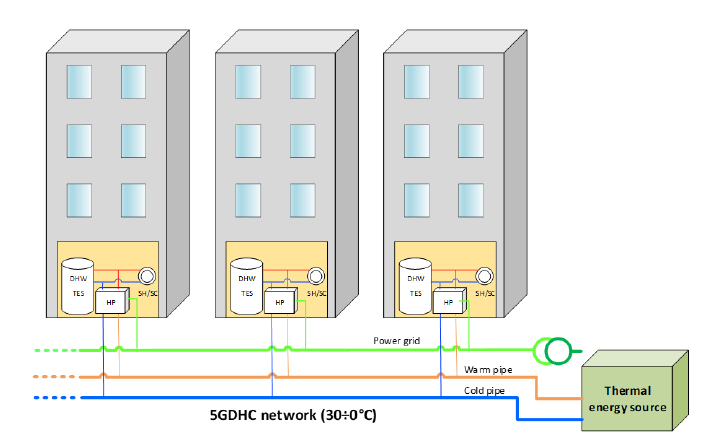
\includegraphics[scale=0.3]{figures/DHC_system.png}
\caption{Layout of a 5GDHC system with decentralized substations and urban excess heat recovery \cite{buffa_fifth-generation_2020}. }
\label{fig:DHC_system}
\end{figure}

The objective of this project is to simulate the implementation of a \gls{ltdhn} system on different localities with different climates. With these simulations on hand companies can decide whether the implementations of these networks can be beneficial both for the future customers and the company itself. This decision depends on multiple factors and variables, for instance, high \gls{cop} values, \idest high ratios between the thermal output and electricity consumption, low heat losses along the network, and low thermal peak power.

These factors, although not simple, can be calculated from distinct sources of data, for instance the air temperature on an hourly basis and by the estimation of the thermal profile, \idest the consumption of \gls{sh} and \gls{dhw} in the whole year of users, in that locality. 

\begin{figure}[ht]
\centering
\includegraphics[width=\linewidth]{figures/process_diagram.pdf}
\caption{Complete workflow to generate data for the simulation of a \gls{ltdhn}. It begins on \textbf{Location} (left-center, purple rhombus) and finishes on \textbf{Thermal Energy from Sources} and \textbf{Electricity Consumption} (right-center, red rectangles). The blue cylinder means the utilization of a dataset (NOAA or \inspire). White rectangles mean processes, these take inputs (entering arrows), generate the data described in its label and move it to another process if required. Green trapeziums mean input data for specific processes.}
\label{fig:project_workflow}
\end{figure}

This project follows the workflow shown in Figure~\ref{fig:project_workflow}, where we start by selecting a region, then, from that region, an specific city with its corresponding air temperature data and thermal profile. At every step, we perform calculations that serve to discriminate and compare the performance of this type of system in each location. In Section~\ref{sec:data-processing} we describe each process and the importance of it towards the final results.

At the end of the workflow, on processes \emph{Thermal Energy from Sources } and \emph{Electricity Consumption}, we have calculated and collected dozens of attributes, on hourly, daily, and seasonal basis, that we use to compare the performance of this system, \eg the heat loss, \gls{cop}, network temperature, are used to discriminate which cities require higher thermal demands but consume less electricity overall. The results are presented on Section~\ref{sec:results}.



\section{Data Sources}

An important part for this project is the availability of air temperature measurements for a certain locality. More specifically, the measurements must be available in an hourly (or shorter) basis as the foundation of this project relies on changes that must be studied from several levels, going from hourly, daily, monthly, until seasonal changes. We found two data sources that comply with the requirements of the project, which are detailed in Section~\ref{subsec:noaa}, and Section~\ref{subsec:inspire}. 

Alternatives to the previous data sources are provided by the \gls{ecad}\footnote{\url{https://www.ecad.eu}} or offered by the different municipalities of Italy, for instance, the Milan municipality provides monthly or daily temperature measurements \footnote{\url{https://dati.comune.milano.it/dataset/ds305-ambientemeteo-temperature-mese-2008-2014}}. However, these do not meet the hourly requirement.

Lastly, an alternative dataset, from the \gls{isac} \footnote{\url{http://www.isac.cnr.it/climstor/CLIMATE_DATA/}}, containing normalized air temperature values from different cities of Italy, with a precision of 30-second measurements between $1961$ until $1990$, was found at the latest stage of this work and could not be included in the project. However, a future work could include this dataset and validate our findings.

\subsection{United States of America hourly temperatures}
\label{subsec:noaa}

\begin{figure}[ht]
\centering
\includegraphics[scale=0.5]{figures/USA cities.png}
\caption{The cities of Miami, Fresno, Olympia, and Rochester located on a political map of the \gls{usa}.}
\label{fig:USA cities}
\end{figure}

We acquired the data from the \gls{noaa} \cite{noaa2010dataset}. The data included information of different cities across the \gls{usa} with respect to their latitude, longitude, stations, air temperature, humidity, and others attributes. For this study we only used the information about the locality of the station and the hourly measurements of air temperature. One characteristic of this dataset is that it comprises the normalized air temperature ranging from $1981$ until $2010$, \idest the dataset does not contain the real value of the temperature on $2010$ but a normalized value of the measured temperatures in that lapse of time.

With respect to the cities utilized in this project, we selected four relatively distant cities with different climates. In Figure~\ref{fig:USA cities} we show the location of these cities on a political map of the \gls{usa}. The list of selected cities in this country is the following:

\begin{itemize}
    \item \textbf{Miami}: located in the state of Florida, southeast of the country.
    \item \textbf{Fresno}: located in the state of California, southwest of the country.
    \item \textbf{Olympia}: located in the state of Washington, northwest of the country.
    \item \textbf{Rochester}: located in the state of New York, northeast of the country.
\end{itemize}

\subsection{Europe hourly temperatures}
\label{subsec:inspire}

\begin{figure}[ht]
\centering
\includegraphics[scale=0.5]{figures/Europe_cities.png}
\caption{The cities of Rome, Madrid, Stuttgart, and London located on a political map of Europe.}
\label{fig:Europe cities}
\end{figure}

We acquired data of cities across Europe from the \inspire project \cite{dipasquale_chiara_2019_3256270}. Similarly as with the \gls{noaa} data source, We used the air temperature of four different cities, each with a different climate. In Figure~\ref{fig:Europe cities}, we show the location of this cities placed over a map of Europe. The list of selected cities in this region is: 

\begin{itemize}
    \item \textbf{Rome}: located in Italy, in south-central Europe.
    \item \textbf{Madrid}: located in Spain, in south-western Europe.
    \item \textbf{Stuttgart}: located in Germany, in central-western Europe.
    \item \textbf{London}: located in the United Kingdom, in north-western Europe.
\end{itemize}

\subsection{Simulation data}
\label{subsec:simulation-data}

In Figure~\ref{fig:project_workflow}, we show that for some processes, there is input data that does not come from previous processes. For instance, when calculating the \emph{Aquifer Well Temperature} we also need to have the aquifer depth, another example is when calculating the \emph{Heat Losses} we need, among the network and ground temperature, to define the piping properties and the network length.

The input data that some processes need, defined by green trapezoids, are part of simulation data. Depending of the type of data, they could be defined by the user, or obtained by other means. For instance, we set the aquifer depth but extracted the \emph{SH/DHW (A)} from the \inspire project \cite{dipasquale_chiara_2019_3256270}.

The values of the different simulation constants for both the USA and Europe data are:
\begin{itemize}
    \item \textbf{SH/DHW (A)}: Obtained from the \inspire project.
    \item \textbf{DHW Profile Distribution (H)}: Obtained from the \inspire project.
    \item \textbf{DHW Temperature (H)}: Constant through the year at $55\degree$C and denoted as $T_{DHW}$.
    \item \textbf{Minimum network temperature}: Minimum required temperature to be sent through the network and denoted as $T_{min}$.
    \item \textbf{Maximum network temperature}: Maximum required temperature to be sent through the network and denoted as $T_{max}$.
    \item \textbf{Aquifer Depth}: Set to $30\ m$ below ground level.
    \item \textbf{Source 1 Schedule}: Working non-stop from Tuesday at 7 until Saturday at 15 each week.
    \item \textbf{Source 1 Temperature}: Set to $23\degree$C and denoted as $T_{S_1}$.
    \item \textbf{Source 2 Schedule}: Working non-stop from Monday at 0 until Tuesday at 15, and from Thursday at 7 until Saturday at 16.
    \item \textbf{Source 2 Temperature}: Set to $29\degree$C and denoted as $T_{S_2}$.
\end{itemize}

\subsubsection{Functional Unit Composition}

With respect to the land extension of these simulations, we considered a \gls{fu} of $1\ km^2$ of urban area with varying numbers of buildings and typologies within it. 

In the current models there are 2 kinds of building typologies that can be selected: \gls{sfh} and \gls{mfh}. The \gls{sfh} and \gls{mfh} models have a fixed geometry for all climates and periods of construction. They have been defined following the common characteristics for European buildings. The \gls{sfh} building model is composed of two storeys with a total of $100\ m^2$ of living area. The \gls{mfh} model corresponds to a reference residential building that has two dwellings per floor, with a total floor area of $500\ m^2$ \cite{dipasquale_chiara_2019_3256270}.

For the purpose of comparing the \gls{ltdhn} performance in different cities, we considered a residential area of $1,600$ \gls{mfh} buildings. This reference area has been already investigated in previous publications for the scenario assessment of low-temperature DH networks, as a typical high-density urban zone \cite{noauthor_home_nodate}.

\section{Data processing}
\label{sec:data-processing}

%As mentioned in Section~\ref{sec:introduction} and as shown in Figure~\ref{fig:project_workflow}, we must perform different calculations based on the air temperature on an hourly basis to determine the feasibility of the implementation of a \gls{ltdhn} in a certain locality. In this section we will describe each process in detail.

The methodology used in this project is a bottom-up approach for the calculation of the total heat demand for \gls{sh} and \gls{dhw} utilization of a district located in 4 different climates across Europe, using data from the \inspire project. The data includes annual energy consumption for each building typology in $kWh/m^2-y$, the selected \gls{sfh} and \gls{mfh} correspond to reference, non-refurbished buildings in each climatic zone built between 1945-1970. In this particular case, the climatic zones and reference cities considered are:

\begin{itemize}
    \item London, United Kingdom: Oceanic climate
    \item Stuttgart, Germany: Continental climate
    \item Madrid, Spain: Southern-dry climate
    \item Rome, Italy: Mediterranean climate
\end{itemize}

Because of lack of specific data available for US cities, we assumed that their characteristic climates are:

\begin{itemize}
    \item Rochester, NY: Continental climate
    \item Olympia, WA: Oceanic climate
    \item Fresno, CA: Southern-dry climate
    \item Miami, FL: Mediterranean climate
\end{itemize}

This calculation is based on the number of \gls{sfh} ($|SFH|$) and \gls{mfh} ($|MFH|$) units. It also depends on the total heat needed by \gls{sfh} ($TOT_{SFH}$) and \gls{mfh} ($TOT_{MFH}$) units. The estimation of the total heated area for buildings within the functional unit ($HD_y$) is shown in Equation~\ref{eq:hd}.

\begin{equation}
\label{eq:hd}
    HD_y = |SFH| \times 100 \times TOT_{SFH} + |MFH| \times 500 \times TOT_{MFH}
\end{equation}

Lastly, based on the climate of the city and using the data collected by the \inspire project, we obtained the demand needed by \gls{sh} ($\%SH_y$) and \gls{dhw} ($\%DHW_y$) with respect of the total heat demand for the year.

\subsection{SH Profile Distribution}

To analyze the performance of this particular \gls{dh} system, it is fundamental to take into account the spatial distribution of the heat demand, but also the distribution over time of it.

For this purpose, the space heating hourly profile for each location is retrieved with a time dependency according to the heating degree method, known as the \emph{Integration method} \cite{deg_days} and calculated as in Equation~\ref{eq:heating_degree}, where $t$ is the current hourly air temperature. 

\begin{equation}
\label{eq:heating_degree}
    HeatingDegree(t)=
\left\{
	\begin{array}{ll}
		15 - t  
		    & \mbox{if } t \leq 15 \\
		0 
		    & otherwise
	\end{array}
\right.
\end{equation}

This method accounts the amount (in degrees) and for how long (in hours) thermal heat is required to keep the indoor building temperature at a comfortable level, which will vary depending on different climates. The base temperature selected was set to $15\ \degree C$.

After the calculation of each degree day, we calculated the distributed heating degree, which is dividing each heating degree measurement by the sum of them in the whole year (see Equation~\ref{eq:dist_heating_degree}).

\begin{equation}
\label{eq:dist_heating_degree}
    DistHeatingDegree(t) = \frac{HeatingDegree(t)}{\sum_{x \in T} HeatingDegree(x)}
\end{equation}

\subsection{SH Consumption (H)}

Now that we obtained both the total heat demand demand for the different cities and that we calculated the distributed heating degrees, obtaining the \gls{sh} Consumption in an hourly basis is:

\begin{equation}
\label{eq:sh_consumption}
    SH(t) = DistHeatingDegree(t) \times \%SH_{y}
\end{equation}



\subsection{DHW Consumption (D)}

Domestic hot water consumption is not influenced by weather and its variation is almost constant over the year. The hourly demand for hot water is estimated by the percentage of hot water ($DHW_y$) inside the total heat demand in the year($HD_y$). This data is also obtained from the \inspire database for different climatic zones. 

\begin{equation}
\label{eq:dhw_d}
DHW(d) = \frac{HD_{y} \times \%DHW_{y}}{d}    
\end{equation}

The total domestic hot water demand is evenly distributed over each day of the year, and then its hourly distribution is obtained by multiplying the daily needs by an hourly random profile. The \gls{dhw} consumption is calculated in a daily basis using Equation~\ref{eq:dhw_d}. 

\subsection{Thermal Load Profile (H)}

Thus, the aggregated heat demand is obtained by adding the thermal heat requirements for SH and DHW. As a result, it is possible to illustrate the different heat load patterns on an hourly basis for a typical high-density residential area located in different cities. Figures \ref{fig:London_thermal_winter} and \ref{fig:London_thermal_summer} show the seasonality effect on the heat load, it is possible to observe the constant pattern in summer that corresponds to only DHW consumption.


The weather dependence of the heat load is shown using a system heat power signature (HPS). A HPS is generated combining the values of thermal demand with the corresponding outdoor temperatures. In \ref{fig:heat_signature_all} we present hourly data, showing a clear linear interdependence between the thermal load and outdoor temperatures for space heating \cite{werner_district_2013}.


It is expected that solar gains through windows are present between 8 - 15\degree C, resulting in a smaller heat load than the line representing the HPS. This is a real-world explanation for using the heating degree day threshold temperature when calculating degree-days.

\begin{figure}[H]
\begin{subfigure}{\textwidth}
\includegraphics[width=0.9\linewidth]{figures/heat_signature_all.png}
\caption{All cities}
\label{fig:heat_signature_all}
\end{subfigure}

\begin{subfigure}{0.5\textwidth}
\includegraphics[width=0.9\linewidth]{figures/london_heat_signature.png}
\caption{London, UK}
\label{fig:heat_signature_london}
\end{subfigure}
\begin{subfigure}{0.5\textwidth}
\includegraphics[width=0.9\linewidth]{figures/stuttgart_heat_signature.png}
\caption{Stuttgart, Germany}
\label{fig:heat_signature_stuttgart}
\end{subfigure}

\begin{subfigure}{0.5\textwidth}
\includegraphics[width=0.9\linewidth]{figures/rome_heat_signature.png}
\caption{Rome, Italy}
\label{fig:heat_signature_rome}
\end{subfigure}
\begin{subfigure}{0.5\textwidth}
\includegraphics[width=0.9\linewidth]{figures/madrid_heat_signature.png}
\caption{Madrid, Spain}
\label{fig:heat_signature_spain}
\end{subfigure}

\caption{Heat power signature for cities in Europe.}
\label{fig:heat_signature_europe}
\end{figure}

\subsection{Climate Curve (H)}

We used a \emph{climatic curve}, which is a tool used to determine the space heating temperature that should be sent through the network based on the outside air temperature. This temperature is bounded within a minimum and maximum desired temperature. In our case, the bounds $T_{min}$ and $T_{max}$ were defined in Section~\ref{subsec:simulation-data}. In Equation~\ref{eq:climatic-curve}, we show the function that we used for the climatic curve, where $t$ is the current hourly air temperature, $m = \frac{T_{max} - T_{min}}{2.38 - 7.25}$, and $b = -m \times 2.38 + T_{max}$. We assumed this values as min and max outdoor temperature levels as reference for the controllers on the buildings side in order to set the max and min indoor temperature levels as shown in Figure \ref{fig:Climatic curve}.

\begin{equation}
\label{eq:climatic-curve}
    ClimaticCurve(t) = 
\left\{
	\begin{array}{lll}
		T_{max}  
		    & \mbox{if } t \leq 2.38 \degree C \\
		T_{min} 
		    & \mbox{if } t \geq 7.25 \degree C\\
		m \times t + b
		    & otherwise \\
	\end{array}
\right.
\end{equation}

\begin{figure}[H]
\centering
\includegraphics[scale=0.4]{figures/Climatic curve.png}
\caption{Average climatic curve implemented in the model. The red dashed line represents a general behavior of several temperature set points of different buildings.}
\label{fig:Climatic curve}
\end{figure}

\subsection{User Temperature Level (H)}
With the calculations that we previously performed, specifically, the space heating value, the climatic curve, and the constant temperature for \gls{dhw} defined in Section~\ref{subsec:simulation-data}, we can calculate the heating temperature that will receive the user on its house, based on the current air temperature, and their corresponding consumption and needs for domestic hot water and space heating. In Equation~\ref{eq:user-temperature}, we show how we calculated the User Temperature Level.

\begin{equation}
\label{eq:user-temperature}
    UserTemperature(t) = \frac{SH_y}{HD_y} \times ClimaticCurve(t) + \frac{DHW_y}{HD_y} \times T_{DHW}
\end{equation}

\subsection{Fitting Curve (H)}
Some processes are not influenced by each reading value in the air temperature, but on the aggregate of these over time. \eg temperature of the ground is not affected by peak changes on air temperature, but on the sustained value of these.

\begin{equation}
\label{equation:fit-curve}
    T_{fit}(t) = \widehat{disp} + \widehat{amp} \times \cos(t \times \omega - \widehat{\phi}) 
\end{equation}

With the aim of estimating an average outdoor temperature, we estimated a curve that fits the data with a reasonable knowledge of its behavior. This is a standard problem in physics in which many processes are periodic: the piston of a motor, the pendulum of a watch, the motion of a wheel, etc. \cite{fitting_curve}. A Python method called "optimize fit" was used which uses non-linear least squares to fit a function as Equation (\ref{equation:fit-curve}) to some input data. 
According to this method, where $\omega = \frac{2 \times \pi}{|H|}$, and $|H|$ is the number of hours in the year. $\widehat{disp}$, $\widehat{amp}$, and $\widehat{\phi}$ represent the \emph{displacement}, \emph{amplitude}, and \emph{phase} of the curve, respectively. These were unknown and dependent from the air temperature of the city. We estimated them using the $scipy.optimize.curve\_fit$ function provided by the SciPy\cite{2020SciPy-NMeth} library.


\subsection{Ground temperature}
With the adjusted temperature ($T_{fit}$) on hand, considering that the network pipes are at $1m$ depth, and using the equation (see Equation~\ref{eq:ground-temperature}) obtained by Kasuda \cite{measurements_of_ground_temperature_at_various_depth}, we calculated the ground temperature and its variation for the entire year in an hourly basis. We set $\alpha = \num{7e-7}$, $T_{sec} = 365 \times 24 \times 3600$, and $d_{min}$ as the day of the year with the minimum recorded temperature.

\begin{multline}
\label{eq:ground-temperature}
    T_{ground}(t, depth) = T_{fit} - \widehat{amp} \times \exp\left( 
        -depth \times \sqrt{ \frac{\pi}{T_{sec} \times \alpha}} \right) \\
    \times \cos\left( 
        \frac{2\pi}{T_{sec}} \times \left( 
            \left(t - d_{min} \times 24\right) \times 3600 -\frac{depth}{2} \times \sqrt{ \frac{T_{sec}}{\pi \times \alpha}}\right)
        \right)
\end{multline}

\subsection{Aquifer Well Temperature (Y)}
\label{subsec:aquifer}

Another important factor for this work is the presence of a nearby aquifer that can be used when no heat is generated by the sources. As we mentioned in Section~\ref{subsec:simulation-data}, we supposed that an aquifer was present in all the cities and that it is located at $30m$ depth. We calculated the aquifer temperature ($T_{aq}$) using Equation~\ref{eq:ground-temperature} with the only change of changing the depth from $1m$ to $30m$.

An interesting result when calculating the aquifer temperatures is that its temperature is constant through the year and is close to the mean yearly air temperature.

\subsection{Network Temperature (H)}

An important attribute of \gls{ltdhn} system is the presence of different sources of heat to feed the system. For this project, we simulated the presence of an aquifer and two different industrial sources ($S_1$ and $S_2$), providing different heat temperatures ($T_{S_1}$ and $T_{S_2}$), and working on different schedules ($S_{S_1}$ and $S_{S_2}$).

\begin{equation}
\label{eq:network-temperature}
    NetworkTemperature(T_{S_1}, T_{S_2}, T_{aq}) = 
\left\{
	\begin{array}{lll}
		T_{aq}  
		    & \mbox{if } T_{S_1} = T_{S_2} = 0 \degree C \\
		T_{S_2} 
		    & \mbox{if }  T_{S_1} = 0 \degree C \mbox{ and } T_{S_2} \neq 0 \degree C \\
		T_{S_1} 
		    & \mbox{if }  T_{S_1} \neq 0 \degree C \mbox{ and } T_{S_2} = 0 \degree C \\
		min(T_{S_1}, T_{S_2})
		    & otherwise \\
	\end{array}
\right.
\end{equation}

\begin{figure}[H]
\centering
\includegraphics[scale=0.5]{figures/Net_temperature.png}
\caption{Sources availability and temperature levels in the \gls{ltdhn}. This pattern is assumed constant along the year.}
\label{fig:Net_temp}
\end{figure}

We calculated the network temperature ($T_{net}$) using the Equation~\ref{eq:network-temperature}, where the temperature of each source is determined by their corresponding working hours, \idest if the source is not producing heat at an hour $t$, then its temperature will be $0$, otherwise its temperature will be either $T_{S_1}$ and $T_{S_2}$, respectively.


\subsection{Coefficient of Performance}

Heat pumps located at the users' substations are responsible for lifting the network temperature to a desired level for \gls{sh} and \gls{dhw} consumptions. The performance of a LTDH system will depend on the operating conditions of the network given by the temperature levels of the sources, and the required temperature levels on the buildings side. Equation~\ref{eq:cop} provides a simplified physical understanding of the effects related to the heat pump performance with a minimum number of parameters:

\begin{equation}
\label{eq:cop}
    COP\ = \eta_{m} COP_{C} +1 - \eta_{m}
\end{equation}

\begin{equation}
COP_{C}= \frac{T_{c}}{T{_c} - T_{e}} 
\end{equation}

\begin{equation}
T_{c}= T_{c,o} +  \Delta T_{HEX} 
\end{equation}

\begin{equation}
T_{e}=  T_{e,o} -  \Delta T_{HEX} 
\end{equation}

Where $COP_{C}$ corresponds to the Carnot COP\cite{grassi_2018} which is a function of the condenser ($ T_{c}$) and evaporator ($T_{e}$) refrigerant temperatures respectively. These variables are estimated as the external fluid outlet temperatures, adjusted by a temperature drop ($\Delta T_{HEX}$) at the heat pump condenser and evaporator.  

\subsection{Heat Losses}

The network properties in the system are specified by the user of the tool. In this particular case, it was assumed a total network length of \SI{2}{\km}, built with pre-insulated pipes which overall heat loss coefficient is U=\SI{0.424}{\W/(m*K)}. As a result, the network losses \SI{0.85}{\kW} of thermal power for every \degree K of temperature: 

\begin{equation}
E_{loss,sup}= U*(T_{net,sup} - T_{gr}) 
\end{equation}

\begin{equation}
E_{loss,ret}= U*(T_{net,ret} - T_{gr}) 
\end{equation}

This means that in winter season when the temperature difference between the network fluid temperature (in the supply or return pipe) and the ground around the pipes ($T_{gr}$) is 15 K, the heat lost in the distribution network is around 12.7 kW.


\subsection{Electricity Consumption}

The hourly \gls{hp} electricity consumption of all substations can be estimated as a function of the total thermal demand and the COP:

\begin{align*}
E_{el} = \frac{E_{th}}{COP}
\end{align*}

\subsection{Thermal Energy From Sources}

District heating systems provide the opportunity to use heat supply from several sources at the same time. In order for this to happen, it is necessary a control system that allows many thermal plants to deliver heat at the same distribution system. In this case, the base load can be supplied by up to two sources of waste heat, with a maximum capacity and temperature levels determined by the user of this tool. A third source consisting in aquifer wells provides heat from a depth of about 30 m when the base load plants are not operating, as well as in peak load conditions. The exact depth of the wells is an input from the user of this tool as well.

The energy produced by each waste heat source is determined by its size, and its daily operation schedule ($E_i$):

\begin{equation}
\label{eq:sources-energy}
\begin{array}{lll}
	E_{s1} = E_{cap1}* E_i  
    & \mbox{for } i =1,24 \\
	E_{s2} = E_{cap2}* E_i  
	& \mbox{for } i =1,24 \\
\end{array}
\end{equation}

The thermal energy delivered by the network, and absorbed on the evaporator side of the  \gls{hp}s ($E_{th,e}$ )is estimated as:

\begin{equation}
E_{th,e} = E_{th}* \left(1-\frac{1}{COP}\right) 
\end{equation}

The total energy produced by all the sources has to account for the thermal losses along the network, the electricity consumption of the network pump ($E_{pump}$), and the heat rejected to the network in the case there is cooling ($E_{cool}$). In the present state of the model, the last two components are not considered:

\begin{equation}
E_{th,net} = E_{th,e} + E_{loss,sup} + E_{loss,ret} + E_{pump} - E_{cool}
\end{equation}

The heat balance equation states that all the aggregated demand has to be satisfied by the available sources. In the case of the ground source ($E_{gs}$), the energy provided to the system corresponds to only the hours in the week in which the \gls{wh} plants are not operating. The main reason behind this choice is because of a higher priority to exploit sources available at a higher temperature  in the network operation:

\begin{equation}
E_{th,net} = E_{s1} + E_{s2}+ E_{gs}
\end{equation}
%\begin{figure}[ht]
%\centering
%\includegraphics[scale=0.5]{figures/London_thermal_winter.png}
%\caption{Seasonality effect on the heat load of the city of London and its relation with respect to the outdoor temperature. Season: winter}
%\label{fig:London_thermal_winter}
%\end{figure}

%\begin{figure}[ht]
%\centering
%\includegraphics[scale=0.5]{figures/London_thermal_summer.png}
%\caption{Seasonality effect on the heat load of the city of %London and its relation with respect to the outdoor temperature. %Season: summer}
%\label{fig:London_thermal_summer}
%\end{figure}

\begin{figure}[h]
\begin{subfigure}{\textwidth}
\includegraphics[width=0.9\linewidth]{figures/London_thermal_winter.png}
\caption{Winter}
\label{fig:London_thermal_winter}
\end{subfigure}

\begin{subfigure}{\textwidth}
\includegraphics[width=0.9\linewidth]{figures/London_thermal_summer.png}
\caption{Summer}
\label{fig:London_thermal_summer}
\end{subfigure}

\caption{Seasonality effect on the heat load of the city of London and its relation with respect to the outdoor temperature}
\label{fig:london_thermal}
\end{figure}

Figure \ref{fig:LDC_Europe} illustrates the heat load duration curve (HLDC) of the cities in Europe. In a HLDC diagram the hourly or daily heat loads are sorted in descending order, with the highest thermal load of the year (winter peaks) located to the left and the lowest to the right (summer nights). The HLD diagram will be different annually depending on the weather conditions, therefore for planning purposes it is recommended to use long-term duration diagrams based on historical data \cite{werner_district_2013}. 

As can be seen in this figure, Rome and Madrid are the cities with the highest thermal peak load, reaching a maximum of 50 and 45 MW respectively, but for a short period of time. For instance, typically peak load plants are very expensive to run, thus, this diagram reveals that these cities require a higher thermal power than Stuttgart and London for at least 2000 hours a year, which results in a more expensive operation. For a more detailed analysis on the hourly distribution of the thermal load, Figure \ref{fig:Europe_heatmap} shows the differences among the cities. London and Stuttgart reach their highest thermal demand of about 30 MW in winter season, which pick typically occurs twice a day (between 7 to 8 am and 12 to 13 pm). The assumed distribution for DHW consumption might strongly influence this output.

This situation reflects that even though the winter season in Northern countries is longer and the outdoor temperature levels are lower than Southern countries, the specific heat demand required by a community located in a less favorable climate can still be lower. Typical explanations for low specific heat use are proper building insulation, new energy efficient windows, and low use of hot water \cite{werner_district_2013}.

\begin{figure}[H]
\centering
\includegraphics[scale=0.8]{figures/LDC_Europe.png}
\caption{Heat load duration curve for cities in Europe}
\label{fig:LDC_Europe}
\end{figure}

\begin{figure}[h]

\begin{subfigure}{0.5\textwidth}
\includegraphics[width=0.9\linewidth]{figures/London-heatmap.png}
\caption{London, UK}
\label{fig:London_heatmap}
\end{subfigure}
\begin{subfigure}{0.5\textwidth}
\includegraphics[width=0.9\linewidth]{figures/Stuttgart-heatmap.png}
\caption{Stuttgart, Germany}
\label{fig:Stuttgart_heatmap}
\end{subfigure}

\begin{subfigure}{0.5\textwidth}
\includegraphics[width=0.9\linewidth]{figures/Rome-heatmap.png}
\caption{Rome, Italy}
\label{fig:Rome_heatmap}
\end{subfigure}
\begin{subfigure}{0.5\textwidth}
\includegraphics[width=0.9\linewidth]{figures/Madrid-heatmap.png}
\caption{Madrid, Spain}
\label{fig:Madrid_heatmap}
\end{subfigure}

\caption{Thermal load by hour of the day in European cities}
\label{fig:Europe_heatmap}
\end{figure}

\clearpage
\section{Results}
\label{sec:results}

The previous estimation of system performance on an hourly basis allows the analysis of heat pumps electricity consumption and the thermal energy produced by each source. In this section we visualize these outputs on an hourly basis.

\subsection{Electricity consumption}

Figures \ref{fig:weekly_electric} and \ref{fig:hourly_electric} present the seasonal patterns of electricity consumption according to the day of the week and the hour of the day respectively. 

As previously discussed, the cities of Rome and Madrid are more affected by the winter season than the other cities, with an average electric power consumption of 4 MW on a weekly basis. In Figure \ref{fig:weekly_electric} is possible to see that the weekly patterns in all cities are similar, with a higher electricity demand on Sundays and a lower demand on Monday.

The reasons of this patterns can be partially explained by Figure \ref{fig:Net_temp}. It was assumed a weekly operation schedule of two plants that were able to recycle heat to the adjacent network within that time frame. On Sundays the available plants are off, and therefore the network operates only at the aquifer wells temperature of 11 \degree C (this situation is represented in the figure on Jan 1st). As a result, the heat pumps have to lift the available temperature from a lower level, explaining a lower performance compared with other days. On the other hand, on Mondays the waste source of higher temperature level is operating (29 \degree C vs 23 \degree C), providing a favorable condition for the overall system.


\begin{figure}[h]
\begin{subfigure}{0.5\textwidth}
\includegraphics[width=0.9\linewidth]{figures/El_weekly_London.png}
\end{subfigure}
\begin{subfigure}{0.5\textwidth}
\includegraphics[width=0.9\linewidth]{figures/El_weekly_Stuttgart.png}
\end{subfigure}

\begin{subfigure}{0.5\textwidth}
\includegraphics[width=0.9\linewidth]{figures/El_weekly_Rome.png}
\end{subfigure}
\begin{subfigure}{0.5\textwidth}
\includegraphics[width=0.9\linewidth]{figures/El_weekly_Madrid.png}
\end{subfigure}
\caption{Weekly electric power pattern by season}
\label{fig:weekly_electric}
\end{figure}

\begin{figure}[h]
\begin{subfigure}{0.5\textwidth}
\includegraphics[width=0.9\linewidth]{figures/El_London.png}
\end{subfigure}
\begin{subfigure}{0.5\textwidth}
\includegraphics[width=0.9\linewidth]{figures/El_Stuttgart.png}
\end{subfigure}

\begin{subfigure}{0.5\textwidth}
\includegraphics[width=0.9\linewidth]{figures/El_Rome.png}
\end{subfigure}
\begin{subfigure}{0.5\textwidth}
\includegraphics[width=0.9\linewidth]{figures/El_Madrid.png}
\end{subfigure}

\caption{Electric power pattern by hour of the day}
\label{fig:hourly_electric}
\end{figure}

\subsection{Thermal Energy From Sources}
It is possible to observe in Figure \ref{fig:London_sources} the energy system in London, UK and the energy contribution of each source to the total thermal demand. The proportions along the year remain the same, as it is assumed a constant operation profile for all the sources. The breakdown by season shows the same pattern by day of the week, with a higher predominance of source 1. This is due to the network control choice which in this case prioritize the use of the waste heat available at a lower temperature. It is also possible to note the operation of the aquifer wells only during the weekends. This situation confirms that operating a system of this kind on a temperature level as low as the aquifer wells has a non-negligible impact in the overall system performance, which effect is even higher in the winter season, as shown in Figure \ref{fig:weekly_electric}.
It is also interesting to note that the average thermal energy required for \gls{dhw} in summer season can be of 2.5 GWh, while in winter this amount can be 6 times higher.

\begin{figure}[H]
\begin{subfigure}{\textwidth}
\includegraphics[width=0.9\linewidth]{figures/London-all-sources.png}
\caption{Monthly energy production by source type}
\label{fig:heat_signature_all}
\end{subfigure}

\begin{subfigure}{0.5\textwidth}
\includegraphics[width=0.9\linewidth]{figures/London-sources-winter.png}
\caption{Winter}
\label{fig:winter_season}
\end{subfigure}
\begin{subfigure}{0.5\textwidth}
\includegraphics[width=0.9\linewidth]{figures/London-sources-spring.png}
\caption{Spring}
\label{fig:spring_season}
\end{subfigure}

\begin{subfigure}{0.5\textwidth}
\includegraphics[width=0.9\linewidth]{figures/London-sources-summer.png}
\caption{Summer}
\label{fig:summer_season}
\end{subfigure}
\begin{subfigure}{0.5\textwidth}
\includegraphics[width=0.9\linewidth]{figures/London-sources-fall.png}
\caption{Fall}
\label{fig:fall_season}
\end{subfigure}

\caption{Thermal energy production by source type in London, UK}
\label{fig:London_sources}
\end{figure}

\clearpage
\section{Conclusions}

The data and results visualizations in this project have been relevant to understand on the one hand the different thermal requirements for \gls{sh} and \gls{dhw} on an annual basis in cities with different climates, and on the other, to assess the performance of a \gls{ltdhn} that could potentially provide the heating service.

It is important to state that the outputs are highly influenced by the boundary conditions set by the user of the model. In this particular project, for example, the data selected for the specific heat demand per unit area in \gls{mfh} buildings located in different climates determined that Southern European cities had a higher thermal load than Northern European cities. This can be observed in Figures \ref{fig:LDC_Europe}, \ref{fig:Europe_heatmap}, \ref{fig:heat_signature_all}.

The heat power signature diagram presented in Figure \ref{fig:heat_signature_all} shows the correlation between the thermal power and outdoor temperature. It is interesting to observe that the selected base temperature of 15 \degree C represents the break point in which the thermal power provided to the buildings is not longer explained by the outdoor temperatures, but only by the \gls{dhw} requirements. In this sense, all the cities have a similar thermal load of about 5 MW.

Although not shown in this report, it is important to state the differences among the US and European databases. The former was characterized by normalized values with a low variance on an hourly basis. In contrast, the European data show a greater variance. As a result, the calculations performed afterwards show some discrepancies.

The data visualization allowed us to understand different thermal requirements given by the total thermal load and its distribution. According to this analysis, the communities located in the cities of Rome and Madrid reach a total thermal peak of around 50 MW, while in the case of Stuttgart and London is about 30 MW as shown on Figure \ref{fig:LDC_Europe}. The higher loads start in November and end in the month of March, with typically two thermal peaks: one in the morning between 7-8am, and the second between 11-12am, as shown in Figure \ref{fig:Europe_heatmap}. This last behavior can be explained by the \gls{dhw} hourly profile implemented which shape has this two peaks.  

Moreover, the visualization of the total electricity used on average by the \gls{hp}s by day of the week and hour of the day allows the user to be aware of when to expect a higher load. As can be seen in Figure \ref{fig:weekly_electric} it is possible to observe that the higher loads in all the cities are on the weekends. This can be explained by the available network temperature that in this case corresponds to the operation of the aquifer wells since the \gls{wh} plants are off. On the other hand, it can be observed on Figure \ref{fig:hourly_electric} a seasonal behavior in all the cities, which hourly profile are almost equivalent in the seasons of Summer and Spring. This can be explained by the overall outdoor temperature that is on average higher than the base temperature chosen to calculate the \gls{sh} consumption in all cities. This effect in the seasons of Fall and Winter can be observed by the higher discrepancies among cities.

Finally, the thermal production from different sources can be observed in Figure \ref{fig:London_sources} for the case of London. The effects of the operation schedule determined initially by the user of the model can be visualized on a weekly basis. It is important to note that this profile remains in the same proportions on average, despite of the seasonality of the thermal energy required by the buildings.






\clearpage
\printbibliography

\end{document}
